\chapter{Способ адаптивного моделирования параметров активной зоны}

\section{Описание способа адаптивного моделирования}

Рассмотренный в главе \ref{method} метод построения оптимального порядка имеет существенный недостаток: в базовой ТА-модели не представлены физические расчеты состояния реактора, подтверждающие безопасность каждого состояния.
Согласно \cite{reactor-calc}, расчеты состояния реактора являются довольно сложной вычислительной задачей.
Для полного расчета всех состояний реактора потребуется проводить расчет для каждого состояния $q$ из множества состояний автомата $Q$, что делает задачу вычислительно невыполнимой.

Однако, можно понизить вычислительную сложность метода, используя обобщенный аппрокисматор.
Нейронные сети могут аппроксимировать непрерывные функции. 
Доказана обобщённая аппроксимационная теорема \cite{neuron-gorban}: с помощью линейных операций и каскадного соединения можно из произвольного нелинейного элемента получить устройство, вычисляющее любую непрерывную функцию с некоторой наперёд заданной точностью. 
Это означает, что нелинейная характеристика нейрона может быть произвольной: от сигмоидальной до произвольного волнового пакета или вейвлета, синуса или многочлена. 
От выбора нелинейной функции может зависеть сложность конкретной сети, но с любой нелинейностью сеть остаётся универсальным аппроксиматором и при правильном выборе структуры может достаточно точно аппроксимировать функционирование любого непрерывного автомата.

В последние несколько лет наблюдается взрыв интереса к нейронным сетям, которые успешно применяются в самых различных областях --- бизнесе, медицине, технике, геологии, физике. 
Нейронные сети вошли в практику везде, где нужно решать задачи прогнозирования, классификации или автоматизации. 
Такой успех определяется несколькими причинами.
\begin{enumerate}
 \item Богатыми возможностями. 
 Нейронные сети --- мощный метод моделирования, позволяющий воспроизводить чрезвычайно сложные зависимости.
 Нейросети нелинейны по своей природе. 
 Кроме того, нейронные сети справляются с <<проклятием размерности>>, которое не позволяет моделировать линейные зависимости в случае большого числа переменных.
 \item Простотой в использовании. 
 Нейронные сети учатся на примерах. 
 Пользователь нейронной сети подбирает представительные данные, а затем запускает алгоритм обучения, который автоматически воспринимает структуру данных. 
 От пользователя, конечно, требуется какой-то набор эвристических знаний о том, как следует отбирать и подготавливать данные, выбирать нужную архитектуру сети и интерпретировать результаты, однако уровень знаний, необходимый для успешного применения нейронных сетей, гораздо скромнее, чем, например, при использовании традиционных методов статистики.\cite{neuron-filatova}
\end{enumerate}

Таким образом, можно предложить следующий способ адаптивного моделирования:
\begin{enumerate}
 \item Рассчитываются обучающее множество для нейронной сети состоящее из вариативных параметров активной зоны и соответствующих им характеристик активной зоны;
 \item Производится обучение искусственной нейронной сети на обучающем множестве;
 \item При поиске оптимального порядка обслуживания используются результаты работы искусственной нейронной сети в качестве предварительных оценок параметров активной зоны;
 \item Предложенный порядок проверяется полным физическим расчетом.
\end{enumerate}

\section{Искусственные нейронные сети прямого распространения}
\subsection{Определение искусственной нейронной сети}

Искусственными нейронными сетями (ИНС) называется совокупность моделей биологических нейронных сетей.
ИНС представляет собой сеть искусственных нейронов, связанных между собой искусственными синаптическими соединениями.
Сеть обрабатывает входную информацию и в процессе изменения своего состояния во времени формирует совокупность выходных сигналов.\cite{COURSE}
Так как ИНС моделирует реальную нейронную сеть, рассмотрим принципы функционирования биологического образца.
Структурной единицей биологической нейронной сети является нейрон (нервная клетка).

\begin{figure}[ht]
\center{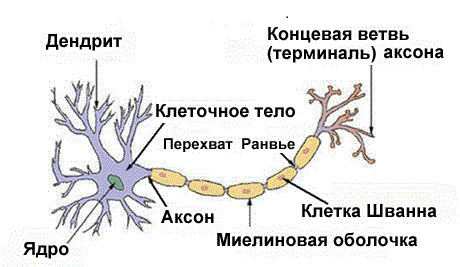
\includegraphics{Neuron.png}}
\caption{Структура нейрона}
\label{ris:neuron}
\end{figure}

Нейрон (рис.~\ref{ris:neuron}) является особой биологической клеткой, которая обрабатывает информацию.
Она состоит из тела клетки, или сомы, и двух внешних древоподобных ветвей: аксона и дендритов.
Тело клетки включает ядро, которое содержит информацию о наследственных свойствах, и плазму, обладающую молекулярными средствами для производства необходимых нейрону материалов.
Нейрон получает сигналы (импульсы) от других нейронов через дендриты и передают сигналы, сгенерированные телом клетки, вдоль аксона, который в конце разветвляется на волокна.
На окончаниях этих волокон находятся синапсы. 
Синапс является элементарной структурой и функциональным узлом между двумя нейронами (волокно аксона одного нейрона и дендрит другого).
Когда импульс достигает синаптического окончания, высвобождаются определенные химические вещества, называемые нейротрансмиттерами.
Нейротрансмиттеры диффундируют через синаптическую щель, возбуждая или затормаживая, в зависимости от типа синапса, способность нейрона-приемника генерировать электрические импульсы.
Результативность синапса может настраиваться проходящими через него сигналами, так что синапсы могут обучаться в зависимости от активности процессов, в которых они участвуют.
Эта зависимость от предыстории действует как память, которая, возможно, ответственна за память человека.
\cite{nn_int_jain}

Созданные из таких структурных элементов биологический нейронные сети обладают следующими свойствами:
\begin{itemize}
\item[-] {\bf Параллельность обработки информации. }
Каждый нейрон формирует свой выход только на основе своих входов и собственного внутреннего состояния под воздействием общих механизмов регуляции нервной системы.
\item[-] {\bf Способность к полной обработке информации. }
Все известные человеку задачи решаются нейронными сетями.
К этой группе свойств относятся ассоциативность (сеть может восстанавливать полный образ по его части), способность к классификации, обобщению, абстрагированию и множество других.
\item[-] {\bf Самоорганизация.}
В процессе работы БНС самостоятельно, под воздействием внешней среды, обучаются решению разнообразных задач.
Неизвестно никаких принципиальных ограничений на сложность задач, решаемых БНС.
Нервная система сама формирует алгоритмы своей деятельности, уточняя и усложняя их в течении жизни.
\item[-] {\bf Надежность. }
Биологические НС обладают фантастической надежностью: выход из строя даже 10\% нейронов в нервной системе не прерывает ее работы. 
По сравнению с последовательными ЭВМ, основанными на принципах фон Неймана, где сбой одной ячейки памяти или одного узла в аппаратуре приводит к краху системы.\cite{COURSE}
\end{itemize}

\subsection{Математические модели работы нейронов}
\subsubsection{Детерминистская модель}
\begin{figure}[ht]
\center{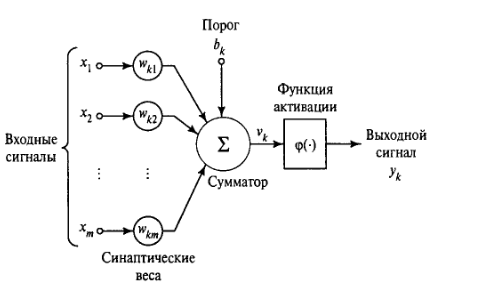
\includegraphics[width=0.8\linewidth]{BlockSheme.png}}
\caption{Явная нелинейная модель нейрона}
\label{ris:BlockScheme}
\end{figure}
Как было выяснено ранее, нейрон представляет собой единицу обработки информации в нейронной сети. 
На блок-схеме рис.~\ref{ris:BlockScheme} показана модель нейрона, лежащая в основе искусственных нейронных сетей.
В этой модели можно выделить три основных функциональных элемента.
\begin{enumerate}
\item Набор синапсов или связей, каждый из которых характеризуется своим весом или силой.
В частности, сигнал $x_j$ на входе синапса $j$, связанного с нейроном $k$, умножается на вес $\omega_{jk}$.
В отличии от синапсов мозга синаптический вес искусственного может принимать как положительные, так и отрицательные значения. 
\item Сумматор складывает входные сигналы, взвешенные относительно соответствующих весов синапсов нейронов.
Математически эту операцию можно описать как линейную комбинацию входных сигналов.
\item Функция активации ограничивает выходную амплитуду сигнала нейрона.
Эта функция также называется функцией сжатия.
Обычно выходной сигнал нормализуется в диапазоне $[0;1]$ или $[-1;1]$.
\end{enumerate}
В модель нейрона, показанную на рис.~\ref{ris:BlockScheme}, включён пороговый элемент, который обозначается символом $b_k$.
Эта величина отражает увеличение или уменьшение входного сигнала функции активации.
В математической форме функционирование нейрона $k$ можно описать следующей парой уравнений:
\begin{equation}
u_k = \sum_{j=1}^{m} \omega_{kj}x_j
\end{equation}
\begin{equation}
y_k = \varphi (u_k + b_k)
\end{equation}
где $x_1,x_2,\dots,x_m$ --- входные сигналы;
$\omega_{k1},\omega_{k2},\dots,\omega_{km}$ --- синаптические веса нейрона $k$;
$u_k$ --- линейная комбинация входных воздействий;
$b_k$ --- порог;
$\varphi()$ --- функция активации;
$y_k$ --- выходной сигнал нейрона.\cite{NejronnyeSeti}
\subsubsection{Функции активации}
Функция активации, представленные в формулах как $\varphi()$, определяет выходной сигнал нейрона.
Можно выделить три основных типов функции активации.
\begin{enumerate}
\item Функция единичного скачка, или пороговая функция.
Этот тип функции описывается следующим уравнением:
\begin{equation}
\varphi(v) = 
\begin{cases}
1, v \ge 0\\
0, v < 0
\end{cases}
\end{equation}
В технической литературе эта форма функции единичного скачка называется функцией Хэвисайда.
Соответственно выходной сигнал нейрона $k$ можно представить как
\begin{equation}
y_k = 
\begin{cases}
1, v_k \ge 0\\
0, v_k < 0
\end{cases}
\end{equation}
где $v_k$ --- индуцированное локальное поле нейрона $k$.
Эту модель в литературе называют моделью Мак-Каллока-Питца. В этой модели выходной сигнал нейрона принимает значение 1 при неотрицательном индуцированном локальным полем, и 0 --- в противном случае.
Это выражение описывает свойство <<все или ничего>> модели Мак-Каллока-Питца.
\item Кусочно-линейная функция. Кусочно-линейная функция описывается следующим выражений:
\begin{equation}
\varphi(v) = 
\begin{cases}
1, v \ge +\frac12\\
|v|, -\frac12<v<+\frac12\\
0, v \le -\frac12
\end{cases}
\end{equation}
где коэффициент усиления в линейной области оператора предполагается равным единице.
Следующие два варианта можно считать особой формой кусочно-линейной функции.
\begin{itemize}
\item [-] Если линейная область не достигает порога насыщения, они превращается в линейный сумматор 
\item [-] Если коэффициент усиления линейной области стремиться к бесконечности, то кусочно-линейная функция выражается в пороговую.
\end{itemize}
\item Сигмоидальная функция. 
Сигмоидальная функция, график которой напоминает букву S, является наиболее распространённой функцией для построения искусственных нейронных сетей.
Это быстрорастущая функция, поддерживающая баланс между линейным и нелинейным поведением.
Примером сигмоидальной функции может служить логистическая функция, задаваемая выражением:
\begin{equation}
\varphi(v) = \frac1{1+e^{-av}}
\end{equation}
где $a$ --- параметр наклона сигмоидальной функции.
Изменяя этот параметр можно построить функции с различной крутизной.
При бесконечно большом параметре наклона функция вырождается в пороговую.
Если пороговая функция принимает только два значения (0 и 1), то сигмоидальная функция принимает бесконечное количество значений в диапазоне $[0;1]$.
При этом сигмоидальная функция является в отличии от пороговой дифференцируемая.\cite{NejronnyeSeti}
\end{enumerate}
\subsection{Топологии нейронных сетей}

Структура нейронных сетей тесно связана с используемыми алгоритмами обучения.
В общем случае можно выделить три фундаментальных архитектуры нейронных сетей.

\subsubsection{Однослойные прямого распространения}

В многослойных нейронной сети нейроны располагаются по слоям.
В простейшем случае у такой сети существует входной слой узлов источника, информация от которого передается на выходной слой нейронов (вычислительные узлы), но не наоборот. 
Такая сеть называется сетью прямого распространения или ациклической сетью.
\begin{figure}[ht]
\center{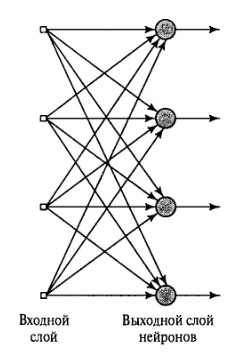
\includegraphics[width=0.4\linewidth]{OneLayer.png}}
\caption{Однослойная сеть прямого распространения}
\label{ris:OneLayer}
\end{figure}

На рис.~\ref{ris:OneLayer} показана структура такой сети для случая четырёх узлов в каждом из слоев (входном и выходном).
Такая нейронная сеть называется однослойной, при этом под единственным слоем подразумевается слой вычислительных элементов (нейронов).
При подсчёте числа слоев мы не принимаем во внимание узлы источника, так как они не выполняют никаких вычислений.\cite{NejronnyeSeti}

\subsubsection{Многослойные прямого распространения}

Другой класс нейронных сетей прямого распространения характеризуется наличием одного или нескольких скрытых слоев, узлы которых называют скрытыми нейронами или скрытыми элементами.
Функция последних заключается в посредничестве между внешним входным сигналом и выходом нейронной сети.
Добавляя один или несколько нейронных слоев мы можем выделить статистики более высокого порядка.
Такая сеть позволяет выделять глобальные свойства данных с помощью локальных соединений за счёт наличия дополнительных синаптических связей и повышения уровня взаимодействий нейронов.
Способность скрытых нейронов выделять статистические зависимости высокого порядка особенно существенна, когда размер входного слоя достаточно велик.

Узлы источника входного слоя сети формируют соответствующие элементы шаблона активации (входной вектор), которые составляют входной сигнал, поступающий на нейроны (вычислительные элементы) второго слоя (т.е. первого скрытого слоя).
Выходные сигналы второго слоя используются в качестве входных для третьего слоя и т.д.
Обычно нейроны каждого из слоев сети используют в качестве входных сигналов только выходные сигналы нейронов предыдущего слоя.
Набор выходных сигналов нейронов последнего слоя сети определяет общий отклик сети на данный входной образ, сформированный узлами источника входного слоя.

\begin{figure}[ht]
\center{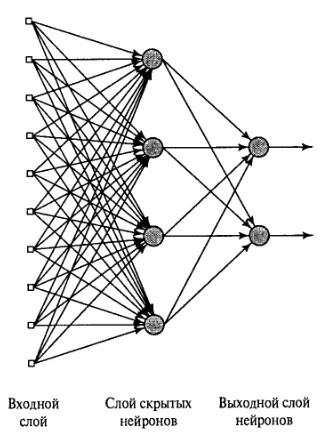
\includegraphics[width=0.4\linewidth]{ManyLayer.png}}
\caption{Многослойная сеть прямого распространения}
\label{ris:ManyLayer}
\end{figure}

Сеть, показанная на рис.~\ref{ris:ManyLayer}, называется сетью 10-4-2, так как имеет 10 входных, 4 скрытых и 2 выходных нейрона.
Нейронная сеть, показанная на рис.~\ref{ris:ManyLayer}, считается полносвязной в том смысле, что все узлы каждого конкретного слоя соединены со всеми узлами смежных слоев.
Если некоторые из синаптических связей отсутствуют, то такая сеть называется неполносвязной.\cite{NejronnyeSeti}

\subsection{Алгоритмы обучения нейронных сетей}

Самым важным свойством нейронных сетей является их способность обучаться на основе данных окружающей среды и в  результате обучения повышать свою производительность.
Повышение производительности происходит со временем в соответствии с определёнными правилами.
Обучение нейронной сети происходит посредством интерактивного
процесса корректировки синаптических весов и порогов.
В идеальном случае нейронная сеть получает знания об окружающей среде на каждой итерации процесса обучения.

С понятием обучения ассоциируется довольно много видов деятельности, поэтому сложно дать этому процессу однозначное определение.
С позиций нейронных сетей мы можем использовать следующее определение обучения
Обучение ---  это процесс, в котором свободные параметры нейронной сети настраиваются посредством моделирования среды, в которую эта сеть встроена.
Тип обучения определяется способом подстройки этих параметров. 

Это определение предполагает следующую последовательность событий при обучении нейронной сети:

\begin{enumerate}
	\item В нейронную сеть поступают стимулы из внешней среды.

	\item В результате этого изменяются свободные параметры нейронной сети.

	\item После изменения внутренней структуры нейронная сеть отвечает на возбуждения уже иным образом.
\end{enumerate}

Вышеуказанный список четких правил решения проблемы обучения называется алгоритмом обучения. 
Несложно догадаться, что не существует универсального алгоритма обучения, подходящего для всех архитектур нейронных сетей.
Существует лишь набор средств, предоставленный множеством алгоритмов обучения, каждый из которых имеет свои достоинства.\cite{NejronnyeSeti}

\subsubsection{Обучение на основе коррекции ошибок}

Для того, чтобы проиллюстрировать первое правило обучения, рассмотрим простейший случай нейрона $k$ --- единственного вычислительного узла выходного слоя нейронной сети прямого распространения.
Нейрон $k$ работает под управлением вектора сигнала $\vec x (n)$, производимого одним или несколькими скрытыми слоями нейронов, которые в свою очередь получают информацию из входного вектора, передаваемого начальным узлам нейронной сети.
Под $n$ подразумевается дискретное время или, более конкретно, --- номер шага итеративного процесса настройки синаптических весов нейрона $k$.
Выходной сигнал нейрона $k$ обозначается $y_k(n)$.
Этот сигнал будет сравниваться с желаемым выходом, обозначенным $d_k(n)$.
В результате получим сигнал ошибки $e_k(n)$.
По определению
\begin{equation}
e_k(n) = y_k(n) - d_k(n)
\end{equation}

Сигнал ошибки инициализирует механизм управления, цель которого заключается применении последовательности корректировок к синаптическим весам нейрона $k$.
Эти изменения нацелены на пошаговое приближение выходного сигнала $y_k(n)$ к желаемому $d_k(n)$.
Эта цель достигается за счет минимизации функции стоимости или индекса производительности $E(n)$, определяемой в терминах сигнала ошибки следующим образом:
\begin{equation}
E(n) = \frac12 e_k^2(n)
\end{equation}
где $E(n)$ --- текущее значение энергии ошибки.
Пошаговая корректировка синаптических весов нейрона $k$  продолжается пока до тех пор, пока система не достигнет устойчивого состояния.
В этой точке процесс обучения останавливается.

Процесс, описанный выше, называется обучением на основе коррекции ошибок.
Минимизация функции стоимости $E(n)$ выполняется по так называемому дельта-правилу, или правилу Видроу-Хоффа, названному в честь его создателей.
Обозначим $\omega_{kj}(n)$  текущее значение синаптического веса $\omega_{kj}$ нейрона $k$, соответствующему элементу $x_j(n)$ вектора $\vec x(n)$, на шаге дискретизации $n$.
В соответствии с дельта-правилом изменение $\Delta\omega_{kj}(n)$, применяемое  к синаптическому весу $\omega_{kj}$ на этом шаге дискретизации, задается выражением
\begin{equation}
\Delta\omega_{kj}(n) = \eta e_k(n)x_j(n)
\end{equation}
где $\eta$ --- некоторая положительная константа, определяющая скорость обучения и используемая при переходе  от одного шага процесса к другому. 
Эту константу естественно именовать параметром скорости обучения.
Вербально дельта-правило можно определить следующим образом:

Корректировка, применяемая к синаптическому весу нейрона, пропорциональна произведению сигнала ошибки на входной сигнал, его вызвавший.

Необходимо помнить, что  определенное таким образом дельта-правило предполагает возможность прямого измерения сигнала ошибки.
Для обеспечения такого измерения требуется поступление желаемого отклика от некоторого внешнего источника, непосредственно доступного для нейрона $k$.
Другими словами нейрон $k$ должен быть видимым для внешнего мира.
Вычислив величину изменения синаптического веса $\Delta\omega_{kj}(n)$, можно определить его новое значение для следующего шага дискретизации:
\begin{equation}
\Delta\omega_{kj}(n+1) = \omega_{kj}(n) +\Delta\omega_{kj}(n)
\end{equation}

\subsection{Парадигмы обучения нейронных сетей}

\subsubsection{Обучение с учителем}

Рассмотрим парадигмы обучения нейронных сетей.
Начнем с парадигмы обучения с учителем.

\begin{figure}[ht]
\center{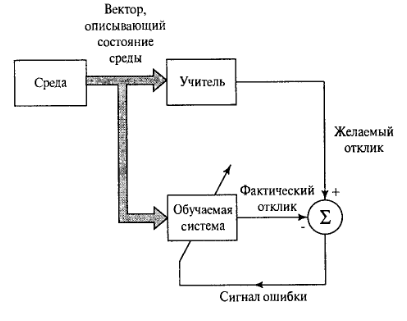
\includegraphics[width=0.6\linewidth]{WithTeacher.png}}
\caption{Блочная диаграмма обучения с учителем}
\label{ris:WithTeacher}
\end{figure}

На рис.~\ref{ris:WithTeacher} приведена блочная диаграмма, иллюстрирующая эту форму обучения. 
Концептуально участие учителя можно рассматривать как наличие знаний об окружающей среде, представленных в виде пар вход-выход.
При этом сама среда неизвестна обучаемой нейронной сети.
Теперь предположим, что учителю и обучаемой сети подается из окружающей среды вектор.
На основе встроенных знаний учитель может сформировать и передать обучаемой нейронной сети желаемый отклик, соответствующий входному вектору.
Этот желаемый результат представляет оптимальные действия, которые должна выполнить нейронная сеть.
Параметры сети корректируются с учетом обучающего вектора и сигнала ошибки.
Корректировка параметров должна выполняться пошагово с целью имитации нейронной сетью поведения учителя.
Эта эмуляция в некотором статистическом смысле должна быть оптимальной.
Таким образом, в процессе обучения знания учителя передаются в сеть в максимально полном объеме.

\clearpage